\documentclass[../main]{subfiles}
\begin{document}
\section{Stiefel-Whitney Number}\label{sec:4.4}

We will now describe a tool which allows us to compare certain Stiefel-Whitney classes of two different manifolds.

Let $M$ be a closed, possibly disconnected, smooth $n$-dimensional manifold. Using mod 2 coefficients, there is a unique \defemph{fundamental homology class}\index{fundamental class!\indexline homology}
\[
\mu_{M} \in \homology_{n}(M ; \, \mathbb{Z} / 2).
\]
(See Appendix~\ref{app:A}.) Hence for any cohomology class $v \in \homology^{n}(M ; \, \mathbb{Z} / 2)$, the \defemphi{Kronecker index}
\[
\ip{v}{\mu_{M}} \in \mathbb{Z} / 2,
\]
is defined. We will sometimes use the abbreviated notation $v[M]$ for this Kronecker index.

Let $r_{1}, \dots, r_{n}$ be non-negative integers with $r_{1}+2 r_{2}+\dots+n r_{n}=n$. Then corresponding to any vector bundle $\xi$ we can form the monomial
\[
\sw_{1}(\xi)^{r_{1}} \cdots \sw_{n}(\xi)^{r_{n}}
\]
in $\homology^{n}(\B(\xi) ;\, \mathbb{Z} / 2) .$ In particular we can carry out this construction if $\xi$ is the tangent bundle of the manifold $M$.

\begin{definition}
\label{def:04.02}
The corresponding integer mod 2
\[
\ip{\sw_{1}(\tangentbundle{M})^{r_1} \cdots \sw_{n}(\tangentbundle{M})^{r_n}}{ \mu_{M}}
\text{ or briefly }
{\sw}_{1}^{r_1} \cdots \sw_{n}^{r_n}[M],
\]
is called the \defemphi{Stiefel-Whitney number} of $M$ associated with the monomial $\sw_{1}^{r_{1}} \cdots \sw_{n}^{r_n}$.
\end{definition}

In studying these numbers, we will be interested in the collection of all possible Stiefel-Whitney numbers for a given manifold. Thus two different manifolds $M$ and $M^{\prime}$ have the same Stiefel-Whitney numbers if 
\[
\sw_{1}^{r_{1}} \cdots \sw_{n}^{r_{n}} [M]=\sw_{1}^{r_{1}} \cdots \sw_{n} ^{r_n}{[M^{\prime}]}
\]
for every monomial ${\sw}_{1}^{r_{1}} \dots \sw_{n}^{r_n}$ of total dimension $n$. (Compare Definition~\pageref{def:06.06} of a partition and \ref{prob:06.04}.)

As an example, let us try to compute the Stiefel-Whitney numbers of the projective space $\projective^{n}$. (which is about the only manifold we are able to handle at this point.) Let $\tau$ denote the tangent bundle of $\projective^{n}$. If $n$ is even, then the cohomology class $\sw_{n}(\tau)=(n+1) a^{n}$ is non-zero, and it follows that the Stiefel-Whitney number $\sw_{n}[\projective^{n}]$ is non-zero. Similarly, since $\sw_{1}(\tau)=(n+1) a \neq 0$, it follows that $\sw_{1}^{n}[\projective^{n}] \neq 0$. If $n$ is actually a power of $2$, then $\sw(\tau)=1+a+a^{n}$, and it follows that all other Stiefel-Whitney numbers of $\projective^{n}$ are zero. In any case, even if $n$ is not a power of $2$, the remaining Stiefel-Whitney numbers can certainly be computed effectively as products of binomial coefficients.

On the other hand if $n$ is odd, say $n=2k-1$, then $\sw(\tau)=(1+a)^{2k}=(1+a^{2})^{k}$, so it follows that $\sw_{j}(\tau)=0$ whenever $j$ is odd. Since every monomial of total dimension $2k-1$ must contain a factor $\sw_{j}$ of odd dimension, it follows that all of the Stiefel-Whitney numbers of $\projective^{2k-1}$ are zero. This gives some indication of how much detail and structure this invariant overlooks.

The importance of Stiefel-Whitney numbers is indicated by the following theorem and its converse.
\begin{theorem}[Pontrjagin]\index{Pontrjagin, L.}
\label{thm:04.09}
If $\base$ is a smooth compact $(n+1)$-dimensional manifold with boundary equal to $M$\index{smooth manifold!\indexline with boundary} (compare \S\ref{ch:17}), then the Stiefel-Whitney numbers of $M$ are all zero.
\end{theorem}

\begin{proof}
Let us denote the fundamental homology class of the pair by
\[
\mu_{\B}\in\homology_{n+1}(\B,M),
\]
the coefficient group $\mathbb{Z}/2$ being understood. Then the natural homomorphism
\[
 \partial:\homology_{n+1}(\B, M)\varrightarrow{} {\homology_{n}(M)}
\]
maps $\mu_{\B}$ to $ \mu_M $. (Compare Appendix~\ref{app:A}.) For any class $v\in \homology^{n}(M)$, note the identity
\[
\ip{v}{\partial\mu_{\B} }=\ip{\delta v}{\mu_{\B}},
\]
where $\delta$ denotes the natural homomorphism from $\homology^{n}(M)$ to $\homology^{n+1}(\B ,M)$. (There is no sign since we are working mod $2$.) Consider the tangent	bundle $\tangentbundle{\B}$ restricted to $M$, as well as the sub-bundle $\tangentbundle{M}$. Choosing a	Euclidean metric\index{Euclidean metric} on $\tangentbundle \B$, there is a unique outward normal vector field along $M$, spanning a trivial line bundle $\trivialbundle^1$, and it follows that
\[
\tangentbundle{\B} |_M\cong\tangentbundle{M}\oplus\trivialbundle^1.
\]
Hence the Stiefel-Whitney classes of $\tangentbundle{\B} $, restricted to $M$, are precisely equal to the Stiefel-Whitney classes $w_j$ of $\tangentbundle{M}$. Using the exact sequence
\[
\homology^n(\B )\varrightarrow{i^\ast}\homology^n(M)\varrightarrow{\delta} \homology^{n+1}(\B,M)
\]
where $i^\ast $ is the restriction homomorphism, it follows that
\[
\delta({\sw}_{1}^{r_{1}} \dots \sw_{n}^{r_n})=0,
\]
and therefore
\[
\ip{({\sw}_{1}^{r_{1}} \dots \sw_{n}^{r_n})}{\partial\mu_{\B} }=\ip{\delta({\sw}_{1}^{r_{1}} \dots \sw_{n}^{r_n})}{\mu_{\B} }.
\]
Thus all Stiefel-Whitney numbers of $M$ are zero.
\end{proof}
The converse, due to Thom, is much harder to prove. 
\begin{theorem}[Thom]\index{Thom, R.}
\label{thm:04.10}
If all of the Stiefel-Whitney numbers
of $M$ are zero, then $M$ can be realized as the boundary of some smooth compact manifold.
\end{theorem}
For proof, the reader is referred to \cite{stongcobordism1968}.

For example the union of two disjoint copies of $M$, which certainly
has all Stiefel-Whitney numbers zero, is equal to the boundary of the
cylinder $M\times [0, 1]$. Similarly, the odd dimensional projective space
$\projective^{2k-1}$ has all Stiefel-Whitney numbers zero. The reader may enjoy trying
to prove directly that $\projective^{2k-1}$ is a boundary.

Now let us introduce the concept of ``cobordism class''.

\begin{definition}\label{def:04.03}\index{cobordism}
Two smooth closed $n$-manifolds $M_1$ and $M_2$ belong
to the same unoriented cobordism class iff their disjoint union $M_1 \sqcup M_2$
is the boundary of a smooth compact $(n+1)$-dimensional manifold.	
\end{definition}

\begin{figure}[ht]
    \centering
    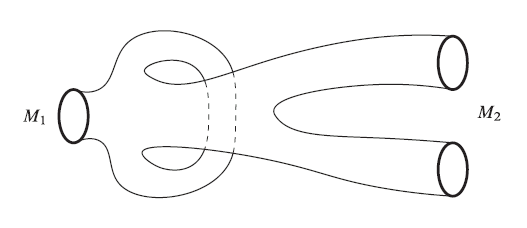
\includegraphics[scale=0.6]{"../tex from old group/fig6.png"}
    \caption{}
    \label{fig:figure6}
\end{figure}


Theorems \ref{thm:04.09}, \ref{thm:04.10} have the following important consequence.
\begin{corollary}\label{cor:04.11}\index{smooth manifold}
Two smooth closed $n$-manifolds belong to
the same cobordism class if and only if all of their corresponding Stiefel-Whitney numbers are equal.	
\end{corollary}
\begin{proof}
The proof is immediate.
\end{proof}

\noindent Here are five problems for the reader.
\begin{problem}
\label{prob:04.01}
Show that the Stiefel-Whitney classes of a Cartesian
	product\index{Cartesian product}\index{Stiefel-Whitney class $\sw_i$} are given by 
	\[\sw_k(\xi\times \eta)=\sum_{i=0}^k \sw_i(\xi)\times \sw_{k-i}(\eta).\]
\end{problem}
\begin{problem}
\label{prob:04.02}
Prove the following theorem of Stiefel. If $n + 1 = 2^r m$ with $m$ odd, then there do not exist $2^r$ vector fields on the projective space $\projective^{n}$ which are everywhere linearly independent.\footnote{Compare \cite{stiefel1936, steenrodwhitehead1951, adams1962}.}\index{vector field}
\end{problem}
\begin{problem}
\label{prob:04.03}
A manifold $M$ is said to admit a field of tangent $k$-planes if its tangent bundle admits a sub-bundle\index{sub-bundle} of dimension $k$. Show that $\projective^{n}$ admits a field of tangent $1$-planes if and only if $n$ is odd. Show that $\projective^{4}$ and $\projective^{6}$ do not admit fields of tangent $2$-planes.
\end{problem}
\begin{problem}
\label{prob:04.04}
If the $n$-dimensional manifold $M$ can be immersed\index{immersion} in $\bR^{n+1}$ show that each $\sw_i(M)$ is equal to the $i$-fold cup product\index{cup product} $\sw_1(M)^i$. If $\projective^{n}$ can be immersed in $\bR^{n+1}$ show that $n$ must be of the form	$2^r-1$ or $2^r-2$.
\end{problem}
\begin{problem}
\label{prob:04.05}
Show that the set $\unorientedCobordism_n$ consisting of all unoriented cobordism classes of smooth closed $n$-manifolds can be made into an additive group. This \defemph{cobordism group} $\mathcal{\unorientedCobordism}_n$ is finite by corollary \ref{cor:04.11}, and is clearly a module over $\mathbb{Z}/2$. Using the manifolds $\projective^{2}\times\projective^{2}$ and $\projective^{4}$, show that $\unorientedCobordism_4$ contains at least four distinct elements.
\end{problem}
\end{document}